\chapter{Środowisko symulacyjne}
\label{sec:model}
W tym rozdziale opisane są stworzone składniki systemu, czyli modele dynamiki i kinematyki, modele czujników oraz pakiety wspomagające testowanie.

Aby uruchomić symulację, nie wystarczy uruchomienie symulatora Gazebo z modelami, należy zadbać także o nadawanie sterowania i odbieranie danych.
Do tego potrzebne są programy wspomagające w formie pakietów ROS, które łączy się w różne konfiguracje, w zależności od scenariusza testowego.
Ze względu na niezależność pakietów od siebie, można ich także użyć przy komunikacji z robotem.

Niektóre typy wiadomości ROS posiadają wbudowany nagłówek, inne istnieją w dwóch wersjach, z nagłówkiem i bez. 
Dopisek \texttt{Stamped} informuje o posiadaniu nagłówka.
Nagłówek ma trzy pola:
\begin{itemize}
	\item Numer sekwencyjny, zwiększany przez program wysyłający po każdej wysłanej wiadomości.
	\item Czas nadania wiadomości, z dokładnością do nanosekund.
	\item Identyfikator macierzy przekształcenia jednorodnego, według której podano dane, ta funkcjonalność została opisana dokładniej w sekcji \ref{sec:frames}.
\end{itemize}

\begin{table}
	\centering
	\begin{tabular}{l r}
		Typ & Opis \\
		\hline
		\texttt{omnivelma\_msgs/Encoders} & Prędkości kątowe i kąty obrotu kół z enkodera. \\
		\texttt{omnivelma\_msgs/Vels} & Prędkości kątowe kół. \\
		\texttt{omnivelma\_msgs/SetFriction} & Nadanie tarcia elementowi modelu. \\
		\texttt{omnivelma\_msgs/SetInertia} & Nadanie mas i momentu bezwładności obiektowi. \\
		\texttt{geometry\_msgs/Pose} & Pozycja obiektu w przestrzeni kartezjańskiej. \\
		\texttt{geometry\_msgs/Twist} & Prędkość względna obiektu. \\
		\texttt{sensor\_msgs/LaserScan} & Jedno skanowanie skanera laserowego. \\
		\texttt{omnivelma\_msgs/Relative} & Odległość i kąt pomiędzy obiektami. \\
		\texttt{nav\_msgs/Odometry} & Pozycja obiektu z macierzą kowariancji. \\
		\texttt{sensor\_msgs/Imu} & Dane generowane przez jednostkę inercyjną. \\
	\end{tabular}
	\caption{Typy wiadomości przekazywanych pomiędzy węzłami.}
	\label{tab:messages}
\end{table}

Węzły można podzielić na trzy typy:
\begin{itemize}
	\item Generujące dane.
	\item Przekazujące filtrujące dane.
	\item Zbierające dane.
\end{itemize}

W tym rozdziale każdy pakiet opisany jest bardziej szczegółowo, wraz z jego interfejsem.
W trakcie testowania symulatora, podłączenie pakietów będzie wyglądać jak na rysunku \ref{uml:final}.

\begin{figure}[H]
	\centering
	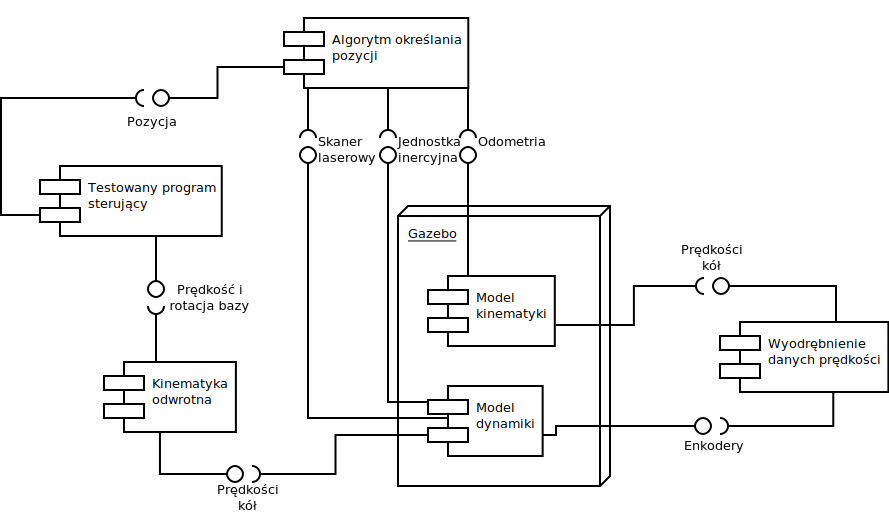
\includegraphics[width=\textwidth]{uml/final.pdf}
	\caption{Komunikacja podstawowych pakietów systemu w trakcie testowania programu sterującego.}
	\label{uml:final}
\end{figure}

Ważną rolę odgrywa tutaj algorytm określania pozycji, bazujący na odometrii, jednostce inercyjnej i danych ze skanera laserowego.
Odometria jest generowana za pomocą modelu kinematyki, sterowanego danymi z enkoderów modelu dynamiki.
Sam model dynamiki sterowany jest pośrednio przez program, który generuje zadane prędkości liniowe i prędkość kątową robota.
W uproszczeniu: program sterujący wysyła sterowanie do modelu, bazując na jego pozycji, określonej z danych generowanych przez modele czujników.

W każdym miejscu przepływu danych można zebrać i zwizualizować przesyłane wartości.
Program sterujący może także korzystać ze skanerów laserowych w celu wykrycia przeszkody, nie tylko w celu określenia pozycji.
Bardziej zaawansowany program sterujący mógłby generować zadane prędkości kół bezpośrednio, nie bazować na modelu kinematyki odwrotnej.

\section{Zapis agentowy}
	Aby zachować kompatybilność programu sterującego platformy mobilnej z jej modelem, należy stworzyć efektory i receptory wirtualne, do których 
	program sterujący będzie wysyłał i z których będzie odbierał dane. 
	Te wirtualne byty będą dalej przekazywać informacje zarówno do modeli, jak i do robota w taki sposób, że
	główny program sterujący nie będzie miał żadnej informacji o tym, do czego jest podłączony. 
	
	\begin{figure}[h]
		\centering
		\includegraphics[width=0.8\textwidth]{graphics/agent.pdf}
		\caption{Struktura agenta upostaciowionego.}
		\label{fig:agent}
	\end{figure} 

	Można to przedstawić za pomocą zapisu agentowego (rysunek \ref{fig:agent}).
	Agent upostaciowiony składa się z kilku modułów, komunikujących się ze sobą za pomocą różnych interfejsów.

	Nadrzędnym modułem jest układ sterowania, który na podstawie odczytów z czujników generuje sterowanie dla efektorów.
	Ważne jest, aby komunikacja z rzeczywistymi urządzeniami była identyczna, jak z ich modelami, dzięki czemu taki system będzie przenośny i niezależny od implementacji modelu.

	Efektor rzeczywisty, na przykład serwomotor, jest sterowany za pomocą efektora wirtualnego, który zamienia wyjście układu sterowania na sygnały sterujące dla silnika napędowego.
	Przykładowo, zmienia odebraną liczbę, oznaczającą zadaną prędkość, na odpowiednie napięcie na wyjściu układu sterującego.

	Zamodelowany efektor symulowany również przyjmuje te same sygnały do układu sterowania, co efektor rzeczywisty, 
	lecz nie zamienia ich na sygnały sterujące, a wywołuje odpowiednie funkcje maszyny symulacyjnej, nadające siły i prędkości obiektom w przestrzeni wirtualnej.

	Receptor wirtualny pobiera surowe dane z czujnika, przekształca na odpowiedni format, usuwa błędy i szum tak, aby program sterujący mógł wykorzystać te dane w prosty sposób. 
	Doskonałym przykładem jest tutaj urządzenie Kinect (widoczne na robocie Velma na rysunku \ref{fig:velma}), w którym to zachodzi odczytanie obrazu z kilku kamer.
	Następnie obraz przesyłany jest do komputera, w którym sterowniki interpretują dane, usuwając błędy, tworzą mapę głębokości, wykrywają szkielety i sylwetki osób.
	Te dane mogą być wykorzystane łatwo w grach i programach sterujących.

	Modelowanie receptora, tak jak w przypadku efektora, polega na wygenerowaniu odpowiednich danych, używając odpowiednich funkcji w przestrzeni wirtualnej.
	Mogą one polegać na emitowaniu półprostych, symulujących laser, lub wręcz renderowaniu obiektów, aby uzyskać obraz z wirtualnej kamery.
	Receptor symulowany ma pełną wiedzę o symulowanym świecie, dokładne położenia i orientacje wszystkich obiektów, dane o kolizjach, itp. 
	Pozwala to na łatwe symulowanie receptorów nie mogących mieć odwzorowania w rzeczywistości, co przydatne jest w pierwszych stadiach testowania i wyznaczaniu statystyk.
	Takim przykładem jest model czujnika dokładnego położenia, orientacji i prędkości w kartezjańskim układzie współrzędnych. 
	Czujniki typu GPS, lub żyroskopy nie generują tak dokładnych pomiarów.


\section{Model kinematyki}
	\label{sec:pseudovelma}
	Kinematyka opisuje ruch obiektów bez rozważania sił powodujących ten ruch.
	Nie uwzględnia się przy opisie ruchu takich czynników jak masa, moment bezwładności, czy siły.
	
	Ten program jest wtyczką symulatora Gazebo oraz modelem w przestrzeni wirtualnej.
	Dzięki temu pozwala na obliczanie i wizualizację pozycji.
	
	Model kinematyki określa równania prostego zadania kinematyki. 
	Rozwiązanie tego zadania polega na obliczeniu prędkości liniowej i kątowej bazy mobilnej na podstawie aktualnych prędkości kół.
	Symulator pozwala również na całkowanie tych prędkości, aby uzyskać aktualną pozycję platformy, z dokładnością do pozycji startowej.
	
	Równania modelu kinematyki najwygodniej przedstawić w postaci macierzowej \cite{wheels}. 
	Dokładna podstać wzoru zależy od kolejności numerowania kół i interpretacji wymiarów.
	Dla opisanego tutaj przypadku, (stałe zdefiniowane są w tabeli \ref{tab:dims}, numeracja kół jest pokazana na rysunku \ref{fig:base_dims}):
	
	\begin{equation}
	\begin{bmatrix}
	v_x \\
	v_y \\
	\omega_z \\
	\end{bmatrix}
	=
	\frac{r}{4}
	\begin{bmatrix}
	-1 & 1 & -1 & 1 \\
	1 & 1 & 1 & 1 \\
	\frac{2}{a+b} & \frac{-2}{a+b} & \frac{-2}{a+b} & \frac{2}{a+b} \\
	\end{bmatrix}
	\begin{bmatrix}
	\omega_1 \\
	\omega_2 \\
	\omega_3 \\
	\omega_4 \\
	\end{bmatrix}
	\end{equation}
	
	Uzyskane wartości należy zastosować w funkcjach symulatora, aby nadać obiektom wirtualnym odpowiednie prędkości.
	
	Sterowanie pozycją modelu kinematyki odbywa się wyłącznie poprzez powyższy wzór, zatem w jego symulacji nie uczestniczy maszyna symulacyjna fizyki.
	Ten model nie reaguje na kolizje z innymi obiektami, nie reaguje na różnicę terenu i nie używa informacji o współczynnikach tarcia materiałów.

	\subsection{Zachowanie}
		Platforma ignoruje inne obiekty znajdujące się na scenie,
		Po nadaniu stałych prędkości kół, następuje ruch zgodnie z rysunkiem \ref{fig:mecanum_dirs}.

		Program sterujący co każdy krok symulacji (okres zależy od zasobów procesorowych komputera) zwraca aktualne położenie i orientację oraz prędkość liniową i kątową obiektu.

\section{Model dynamiki}
	\label{sec:omnivelma}
	Maszyna do symulacji fizyki używa informacji o kształtach, masach i złączach pomiędzy ogniwami robota.
	Należy zatem stworzyć obiekt, złożony z modeli ogniw, i umieścić w symulatorze.
	Wtyczka Gazebo będzie nadawać prędkość kątową kołom i odczytywać dane z czujników.
	Potem należy nadać przegubom odpowiednie siły, aby otrzymać wyniki przybliżone do tego, jak zachowywałaby się rzeczywista baza mobilna.

	Baza mobilna jest bryłą, na którą składają się następujące części składowe:
	\begin{itemize}
	\item Główna część korpusu.
	\item Ruchoma, mniejsza część korpusu, z przodu robota.
	\item 4 koła, 2 podłączone do głównej części korpusu, a 2 do przedniej.
	\item Po 12 rolek na każdym kole.
	\item Przegub obrotowy, łączący dwie części korpusu.
	\item 4 przeguby obrotowe z silnikami, łączące części bazy z kołami.
	\item 12 przegubów obrotowych na każdym kole, łączących koła z rolkami.
	\item Dwa skanery laserowe, przytwierdzone do głównej części korpusu.
	\item Mała jednostka inercyjna.
	\end{itemize}

	Jest to dość złożony obiekt do symulacji, dlatego należy dążyć do uproszczenia modelu w celu zmniejszenia ilości obliczeń symulatora.
	Istnieje wiele podejść do stworzenia odpowiedniego modelu, na przykład jak najdokładniejsze odwzorowanie budowy platformy 
	za pomocą wzorów różniczkowych \cite{braking} \cite{modelling_ways}.
	
	Dodatkową funkcjonalnością jest brak nadawania prędkości kołom w przypadku odebrania pakietu zawierającego ciche nie-liczby (NaN).
	To jest charakterystyczne tylko dla modelu platformy (patrz sekcja \ref{sec:model_nan}).
	
	W tym przypadku umieszczono model o odpowiednich parametrach w symulatorze, aby jego maszyna do symulacji fizyki obliczała prędkości i pozycje obiektów.
	Sam pakiet nie posiada modelu jednostki inercji i skanerów laserowych, a importuje je z innych pakietów.
	
	\subsection{Zachowanie}
		Model reaguje na siły przyłożone do jego ogniw, porusza się, reagując na otoczenie.
		Bierze udział w kolizjach, nadaje prędkości innym obiektom.
		Współczynniki tarcia podłoża i kół mają znaczenie w symulacji.
		Powstają niedokładności wyznaczania pozycji, spowodowane dużą ilością zmiennych, uczestniczących w symulacji i precyzją symulatora.
		
		Zachowanie modelu silnie zależy od jego parametrów, a zwłaszcza od mas i momentów bezwładności ogniw.
	
\section{Model skanera laserowego}
	\label{sec:monokl}
	Symulator generuje odpowiednie dane, emitując promienie w przestrzeni wirtualnej.
	Następnie maszyna symulacyjna fizyki oblicza kolizje promieni z obiektami na scenie, biorąc pod uwagę także ich albedo, sprecyzowane w parametrach modelu. 
	Jest to operacja bardzo kosztowna obliczeniowo.
	
	Do położeń punków dodawany szum o rozkładzie normalnym, aby symulować błędy pomiarowe, powstałe przy odczycie odbicia lasera.
	Model symuluje zarówno pomiary odległości od obiektu, jak i ich intensywność.
	
	Odczyt z rzeczywistego skanera pokazuje, że sztucznie wygenerowane dane są podobne do danych zebranych przez czujnik.

	\begin{figure}[h]
	\centering
	\includegraphics[width=\textwidth]{graphics/scan.png}
	\caption{Zrzut ekranu platformy z Gazebo i wygenerowane dane, obserwowane w Rviz.}
	\label{fig:scan}
	\end{figure}
	
	Ten pakiet składa się z wtyczki obsługującej model skanera i pliku opisującego parametry samego skanera, jak i również wygląd fizyczny, kształt, masę, moment bezwładności obudowy.
	Dane z tego pakietu importowane są przez pakiet modelu dynamiki i umieszczane w odpowiednim miejscu modelu robota z odpowiednim przegubem.
	
\section{Model jednostki inercyjnej}
	Rzeczywisty czujnik obarczony jest bardzo dużymi błędami pomiarowymi.
	Model symuluje przyspieszenie oraz prędkość kątową robota.
	Dodaje sztuczny szum do wygenerowanych danych, aby przybliżyć zachowanie modelu do jednostki inercyjnej.
	
	Niestety, ponieważ ten czujnik jest bardzo czuły na drgania robota, nie wszystkie jego cechy da się poprawnie zasymulować.
	Dodatkowo, wygenerowane dane w dużym stopniu zależą od momentów bezwładności ogniw robota.
	
	Podobnie, jak pakiet modelu skanera laserowego, jest on zaimplementowany jako model umieszczany w symulacji i wtyczka, importowane przez model dynamiki.
	
\section{Model kinematyki odwrotnej}
	\label{sec:transmutator}
	Model kinematyki odwrotnej jest przeciwieństwem modelu kinematyki, opisanego w sekcji \ref{sec:pseudovelma}.
	Ten program przyjmuje prędkość liniową i kątową platformy, następnie oblicza prędkości kątowe kół, wymagane aby nadać platformie zadaną prędkość.
	
	Ten model działa bez symulatora, jako węzeł ROS, filtrujący wiadomości i nie posiada możliwości całkowania wygenerowanych prędkości.
	Całkowanie prędkości kół i tak nie ma większego sensu, ponieważ pozwoliłoby to jedynie obliczyć ich aktualny kąt obrotu.
	Z wyjątkiem porównania tych danych z danymi z enkoderów, nie ma to innego zastosowania.
	
	Wzory kinematyki odwrotnej mogą być przedstawione w postaci macierzowej \cite{wheels} (stałe zdefiniowane są w tabeli \ref{tab:dims}, numeracja kół jest pokazana na rysunku \ref{fig:base_dims}).
	
	\begin{equation}
	\begin{bmatrix}
	\omega_1 \\
	\omega_2 \\
	\omega_3 \\
	\omega_4 \\
	\end{bmatrix}
	=
	\frac{1}{r}
	\begin{bmatrix}
	1 & -1 & \frac{a+b}{2} \\
	1 & 1 & -\frac{a+b}{2} \\
	1 & -1 & -\frac{a+b}{2} \\
	1 & 1 & \frac{a+b}{2} \\
	\end{bmatrix}
	\begin{bmatrix}
	v_y \\
	v_x \\
	\omega_z \\
	\end{bmatrix}
	\end{equation}

	Dodatkowo, program pozwala na obrót wektora wejściowej prędkości o kąt prosty lub półpełny. 
	Jest to spowodowane tym, że różne pakiety i różne modele robotów przyjmują różną orientację wyjściową robota.
	Czasami przód modelu skierowany jest w dodatnią stronę osi X, a czasami Y. W związku z tym, ta funkcjonalność jest w stanie przekonwertować dane wejściowe dla innego robota tak,
	aby mogły być użyte do sterowania modelem platformy.
	

\section{Manualne sterowanie}
\label{sec:lalkarz}
	To zaawansowany program do manualnego generowania zadanych prędkości kół lub prędkości liniowej i kątowej platformy.
	Zaimplementowany jako pakiet ROS.
	Ponieważ jest niezależny od reszty systemu, może być użyty do sterowania rzeczywistym robotem.
	Pozwala także na wyświetlanie aktualnych prędkości kół, generowanych przez enkodery.
	
	Sterowanie można nadać poprzez klawiaturę, kontroler do gier lub myszkę.
	Program otwiera graficzne okno, w którym wyświetla aktualne dane i wskaźniki prędkości.
	
	\subsection{Tryby działania}
		Program posiada 11 trybów działania, w których generuje różne wiadomości w różny sposób.
		Globalny mnożnik wyjścia pozwala na łatwe ograniczenie generowanych danych i ustawienia dokładności. Naciśnięcie klawisza spacji awaryjnie zeruje wszystkie wyjścia.
		\begin{enumerate}
			\item Za pomocą ośmiu klawiszy klawiatury numerycznej, można nadać platformie określone prędkości kół.
			W tym trybie koło może albo stać w miejscu, albo obracać się z odpowiednią prędkością kątową.
			Takie sterowanie powoduje poślizgi platformy. W trakcie braku aktywności użytkownika, generowane jest zerowe sterowanie.
			\item Podobnie do poprzedniego trybu, lecz przy braku naciśnięcia klawisza, generuje cichą nie-liczbę, aby zachować aktualną prędkość kół modelu.
			Ta dodatkowa funkcjonalność opisana jest szerzej w sekcji \ref{sec:model_nan}.
			\item Naciśnięcie klawisza płynnie zwiększa lub zmniejsza prędkość koła. W trakcie braku aktywności użytkownika, generowane jest stałe sterowanie, bazujące na aktualnym ustawieniu programu.
			\item Podobnie, co w poprzednim trybie, lecz pozwala na schodkowe ustawienie prędkości kół co 0,1 \si{\radian\per\second} (pomnożone przez mnożnik wyjścia).
			Dzięki temu możliwe jest w miarę dokładne powtórzenie manualnych testów platformy.
			\item Poprzedni tryb, lecz przy ustawieniu prędkości zerowej, generuje nie-liczbę.
			\item Sterowanie prędkościami kół za pomocą gałek kontrolera.
			Większość kontrolerów posiada dwa, dwuosiowe joysticki, co daje cztery osie, zmieniające się w zakresie $\left<-1;1\right>$.
			Można za ich pomocą bezpośrednio ustawiać prędkości kół. Ten tryb jest nieintuicyjny w działaniu.
			\item Ten tryb generuje zadaną prędkość liniową i kątową, a nie prędkości kątowe kół, jak poprzednie tryby.
			Za pomocą klawiatury można nadać platformie jeden z ośmiu kierunków poruszania się i jeden z dwóch kierunków obrotu wokół osi Z.
			Ta metoda sterowania powoduje skoki prędkości i poślizgi. Przypomina sterowanie pojazdami w grach komputerowych.
			Puszczenie klawiszy powoduje zatrzymanie się platformy.
			\item Podobny tryb do poprzedniego, ale naciśnięcie klawisza płynnie dodaje wartość do prędkości liniowej i kątowej platformy
			Brak aktywności użytkownika powoduje, że generowane jest stałe sterowanie.
			\item Schodkowe sterowanie prędkością platformy w krokach co 0,1 \si{\metre\per\second}. Pozwala na ustawienie prędkości i obrotu platformy z zadaną dokładnością
			i dokładniejsze manualne przeprowadzanie testów.
			\item Sterowanie prędkością liniową i kątową platformy za pomocą kontrolera. Trzy osie są używane, dwie do nadania prędkości liniowej, jedna do nadania prędkości kątowej.
			Jest to prawdopodobnie najczęstszy sposób kontrolowania robotów wielokierunkowych za pomocą kontrolera.
			Sposób bardzo intuicyjny i używany także przez inne pakiety do manualnego sterowania robotami na kołach Mecanum.
			\item Sterowanie za pomocą myszki, najdokładniejsze sterowanie zadaną prędkością liniową i kątową robota.
			Kursor myszy wskazuje końcówkę strzałki reprezentującej kierunek ruchu robota, za pomocą kółka można ustawiać zadaną prędkość kątową robota wokół osi Z.
			Ponieważ większość myszek ma skokowe obroty kółek, wprowadza to nieznaczne poślizgi w nadawanej prędkości kątowej. 
			Można także modyfikować tę wartość klawiaturą w płynnym trybie przyrostowym.
		\end{enumerate}
	
	\begin{figure}[H]
	\centering
	\includegraphics[width=\textwidth]{graphics/lalkarz.png}
	\caption{Zrzuty ekranu dwóch trybów działania programu.}
	\label{fig:lalkarz}
	\end{figure}
	
	Interfejs graficzny (patrz rysunek \ref{fig:lalkarz}) składa się z listy trybów, wyświetlanych na górze, i nazwy aktualnego trybu.
	Wyszarzone tryby nie mogą być aktywowane, w tym przypadku z powodu braku podłączenia kontrolera.
	
	Na lewym zrzucie widać zarys platformy i białe wskaźniki aktualnych prędkości kół, wraz ze współczynnikiem wypełnienia.
	Obok nich znajdują się szare wskaźniki prędkości kątowych kół, zwrócone przez modele enkoderów.
	Małe, szare znaki to nazwy klawiszy, używanych w tym trybie do modyfikowania prędkości.
	
	Na prawym rysunku jest tryb generowania kierunku i obrotu. Strzałka wskazuje wektor prędkości liniowej, a górny pasek prędkość kątową platformy.
	
	Na dole jest lista ,,biegów'' urządzenia, są to zwyczajne mnożniki wyjścia w celu wygodnego przestawiania dokładności z jaką platforma powinna się poruszać.
	
	Wszystkie dane są w jednostkach SI, tzn, efektywna prędkość koła będzie się równać liczbie podanej przy kole, pomnożonej przez aktualny bieg.
	Dla obrotów to są \si{\radian\per\second}, dla prędkości to \si{\metre\per\second}.
	
	Jeszcze jeden parametr pozwala na ustawienie częstotliwości z jaką wysyłane mają być wiadomości przez strumień komunikacyjny.
	
\section{Generator sterowania}
	\label{sec:gramofon}
	Podstawą przeprowadzania testów modelu jest powtarzalność eksperymentów oraz dokładność nadanego sterowania.
	Potrzeba zatem jest sposobu na automatyczne wygenerowanie przesyłanych wiadomości z określonymi danymi.
	
	Ten pakiet ROS generuje powtarzalne sterowanie, bazując na wczytanym pliku tekstowym i podanej częstotliwości wysyłania pakietów.
	Wyjściem są zadane prędkości liniowe i prędkość kątowa bazy.
	
	Dane zapisane są w formie wierszy, w którym każdy określa czas i dane, które program ma nadawać.
	Po zakończeniu wykonywania instrukcji, węzeł generuje wiadomość o zerowych parametrach w celu zatrzymania bazy.
	
		
\section{Wyłuskanie podwiadomości}
	\label{sec:dziadzio}
	Każda wiadomość przekazywana pomiędzy węzłami jest zwykle zagnieżdżoną strukturą.
	Ten pakiet ROS działa jak filtr dla strumienia wiadomości.
	
	Czasami może zdarzyć się, że jakiś węzeł potrzebuje jedynie wewnętrznej podstruktury wiadomości.
	Mógłby subskrybować całą wiadomość, lecz to powodowałoby potrzebę przesyłania dodatkowych, nieużywanych danych oraz nie pozwoliłoby na zachowanie niezależności pakietu od innych.
	
	Takie zjawisko występuje przy przekazywaniu informacji o prędkości kątowej i kącie obrotu kół, generowanej przez model czujnika enkoderów, do programu
	manualnego sterowania lub do modelu kinematyki. 
	
	ROS nie pozwala na automatyczne przesłanie tylko części pakietu pomiędzy węzłami, dlatego powstał ten program.

\section{Podłoże o zmiennym współczynniku tarcia}
	\label{sec:flooria}
	Symulacja nie składa się jedynie z robota i czujnika, ale także z podłoża, na którym musi się poruszać.
	Ponieważ podłoże również wpływa na symulację, powinien istnieć sposób na ustawienie jego współczynnika tarcia.
	
	Ten pakiet jest modelem ładowanym do symulatora Gazebo, przyjmuje on asynchroniczne wywołania, nadające podłożu odpowiednie tarcie.
	W ten sposób można testować zachowanie się modelu w różnych przypadkach testowych.
	
\section{Algorytm usuwania szumu z danych jednostki inercyjnej}
	\label{sec:odszumiacz}
	Jak wcześniej wspomniano, jednostka inercyjna i jej model zwracają bardzo duże błędy pomiarowe.
	
	Ten filtr uśrednia dane w prosty sposób, licząc średnią z określonej ilości poprzednich pomiarów.
	Działa to bardzo dobrze przy uśrednianiu szumu przy zerowym przyspieszeniu lub w trakcie ruchu robota z prędkością jednostajną.
	Nie sprawdza się jednak przy odczycie faktycznego przyspieszenia, gdyż może generować zaniżone wartości.
	
	W przyszłości zastosować trzeba będzie bardziej zaawansowany algorytm uśredniania odczytów.
	Może on być również testowany na tym modelu.
	
	Stworzenie tego programu pozwoliło zbadać, czy model jednostki inercyjnej oraz jednostka inercyjna platformy reagują na ruch w odpowiednim kierunku, gdyż
	pomiary są obarczone tak dużymi błędami, że wizualizacja odczytów na wykresie nie daje gwarancji upewnienia się o działaniu modelu.
	
\section{Obserwator symulacji}
	\label{sec:ocznica}
	Wtyczka uruchamiana w symulatorze.
	Oblicza i zwraca statystyki międzymodelowe w przestrzeni symulacji, takie jak odległość i kąt.
	Pozwala zbadać, jak model dynamiki zachowuje się w stosunku do modelu kinematyki, to znaczy, 
	czy pozycja, obliczona przez maszynę symulacyjną fizyki jest zbliżona do pozycji obliczonej równaniami kinematycznymi po scałkowaniu.
	
\section{Scena z symulacją}
	Symulator Gazebo przy uruchomieniu ładuje plik opisujący symulację.
	Ten pakiet nie jest programem wykonywalnym, a zestawem kilku plików czytanych przez Gazebo.
	W tych plikach zawierają się także ustawienia symulacji, jak przyspieszenie grawitacyjne, typ maszyny symulacyjnej fizyki ze współczynnikami, czy ustawienia wirtualnej atmosfery.
	
	Zapisane są tutaj nazwy modeli importowanych z innych pakietów.
	
\section{Rozdzielacz wiadomości}
	Jeśli dwóm węzłom nadać te same nazwy interfejsów strumienia wiadomości, to ROS będzie przekazywał pomiędzy nimi informacje.
	To jednak nie zawsze jest możliwe, aby mieć całkowitą kontrolę nad nazwami interfejsów wszystkich węzłów.
	Dlatego też, potrzebny jest program do przekazywania i ewentualnego rozdzielania wiadomości dla różnych odbiorników.
	
	Ten program wykonywalny pobiera i generuje wiadomości zawierające zadane prędkości kół.
	Pozwala to na sterowanie kilkoma robotami o identycznym interfejsie ze wspólnego źródła.
	W szczególności przydaje się to przy rozdzielaniu wartości prędkości kół dla modelu platformy dynamiki i kinematyki.
	
	Ten pakiet może być zastąpiony przez kilkukrotne uruchomienie wbudowanego w ROS narzędzia \texttt{relay}, które przekazuje pakiet z jednego strumienia komunikacyjnego do innego.
	
\section{Prosty program sterujący}
	Jest to uproszczona wersja programu, który docelowo ma być tworzony na podstawie budowanego systemu modeli.
	
	Program periodycznie wysyła dane o zadanej prędkości, zależnej od aktualnego stanu.
	W zależności od danych ze skanerów laserowych, program zmienia swój stan i obraca kierunek obrotu o \ang{90}.
	Ten sterownik dla uproszczenia nie generuje poleceń obrotu kątowego, sterowany obiekt powinien zachować swoją orientację.
	
	Prosty algorytm programu gwarantuje omijanie przeszkód, jednak nie bierze pod uwagę celu jazdy.
	To znaczy, że platforma będzie poruszać się od przeszkody do przeszkody w losowy sposób.
	
\section{Struktury pakietów wiadomości}
	Ten pakiet nie jest plikiem wykonywalnym, a definicjami struktur danych, używanymi przez wiadomości ROSa w projekcie, jeśli 
	standard nie obejmuje potrzebnego typu wiadomości.
	
	Dodatkowo zdefiniowane typy wiadomości to:
	\begin{itemize}
		\item Dane prędkości kątowej i kącie obrotu kół, zwracane przez model enkoderów.
		\item Dane o względnym położeniu i orientacji obiektów na scenie.
		\item Zadane prędkości kątowe kół.
		\item Asynchroniczne wywołanie do ustawienia mas i momentów bezwładności ogniw modelu.
		\item Asynchroniczne wywołanie do ustawienia współczynników tarcia obiektu.
	\end{itemize}

\section{Zewnętrzne pakiety ROSa}
	Istnieje kilka tysięcy różnych pakietów i programów, tworzonych przez społeczność ROSa.
	Te zostały użyte w projekcje.
	
	\subsection{Rysownik wykresów}
		Pakiet \texttt{rqt-multiplot} jest wtyczką do większego programu \texttt{rqt}.
		Pozwala na generowanie dwuwymiarowych wykresów, bazując na dwóch dowolnych wartościach z odbieranych pakietów, łącznie z czasem nadania.
		Pozwala porównać różne wykresy na jednym układzie.
		
		W szczególności, przy ustawieniach wyświetlania składowych położenia Y względem X, pobranych z pakietu pozycji, pozwala narysować trajektorię ruchu platform.
		
	\subsection{Wizualizer pomiarów}
		Oryginalnie napisany dla robota o tej samej nazwie, \texttt{rviz} prezentuje trójwymiarową przestrzeń, w której można wyświetlać 
		dane odebrane z innych węzłów.
		
		Pozwala to na przykład umieścić znacznik reprezentujący pozycję platformy i chmury punktów, odebranych ze skanerów laserowych.
		Jest lżejszy na zasobach w działaniu niż Gazebo i pokazuje tylko informacje z odebranych danych, a nie całe środowisko symulacji.
		Nie posiada własnego symulatora fizyki, nie generuje żadnych danych samodzielnie.
		
	\subsection{Algorytm określania lokalizacji}
		Pakiet \texttt{laser\_scan\_matcher} pozwala na określenie pozycji robota, bazując na danych ze skanera laserowego oraz opcjonalnie jednostki inercyjnej i enkoderów w
		celu minimalizacji błędów. Bazuje na porównywaniu kolejnych odczytów chmury punktów pomiarowych.
		Istnieją bardziej zaawansowane algorytmy określania pozycji, na przykład bazujące na modelu mapy, lecz ten pakiet jest prosty w użyciu i nie wymaga dodatkowych danych, ani kalibracji.
		
	
	
	
	
	

